\documentclass{scrartcl}
\usepackage{german}
\usepackage[T1]{fontenc}
\usepackage[utf8]{inputenc}
\usepackage[german]{babel}

% zusätzliche mathematische Symbole, AMS=American Mathematical Society
\usepackage{amssymb}

% fürs Einbinden von Graphiken
\usepackage{graphicx}

% für Namen etc. in Kopf- oder Fußzeile
\usepackage{fancyhdr}

% erlaubt benutzerdefinierte Kopfzeilen
\pagestyle{fancy}

% Definition der Kopfzeile
\lhead{
	\begin{tabular}{ll}
		Fisnik Zeqiri & 4306430 \\
		Felix  Karg   & 4342014
	\end{tabular}
}
\chead{}
\rhead{\today{}}
\lfoot{}
\cfoot{Seite \thepage}
\rfoot{}

\begin{document}
	\section*{Antworten zum Übungsblatt Nr. 4}
	
	\subsection*{Aufgabe 1}
	
	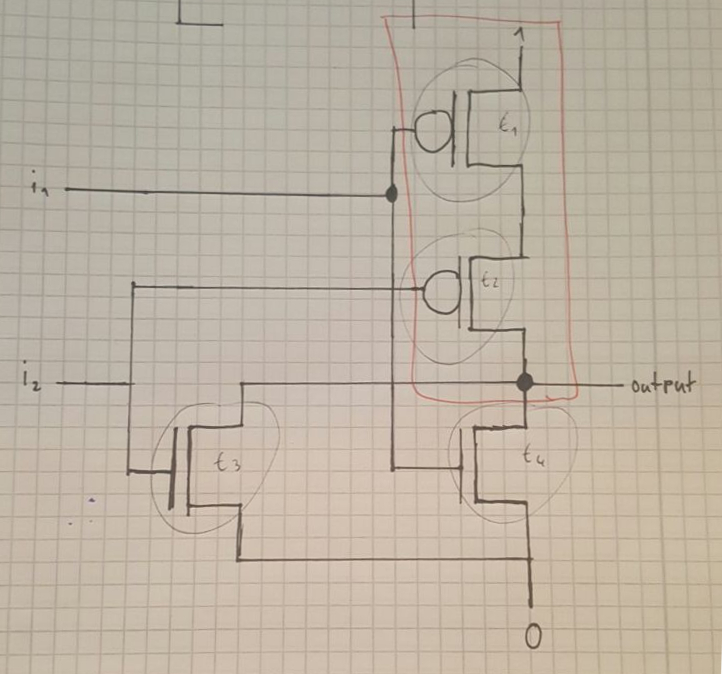
\includegraphics[width=14cm]{bild1.jpg}
	
	[Bild 1]\\\\
	Funktion: Der NOR-Gatter ist nur dann 1, wenn beide Inputs 0 sind. Ist dies der Fall, sperren t3 und t4. Da t1 und t1 leiten, fließt die logische 1 zum Output und das Ergebnis ist 1.
	In allen anderen Fällen ist mindestens ein Input i1, weshalb die Logische 0 mit dem Output verbunden ist.\\
	Der im Bild rot markierte Bereich verbindet die Logische 1 mit dem Output. Die Leitung besteht nur dann, wenn beide Transistoren leiten. Dies ist nur der Fall, wenn beide Inputs 0 sind.
	
	
	\subsection*{Aufgabe 2}
	\begin{itemize}
		\item[a)] Zuerst erstellen wir eine Wahrheitstabelle:\\
		\begin{table}[h]
			\begin{tabular}{l|l|l|l}
				x1 & x2 & x3 & $x1\oplus x2\oplus x3$ \\ \hline
				0  & 0  & 0  & 0 \\
				0  & 0  & 1  & 1 \\
				0  & 1  & 0  & 1 \\
				0  & 1  & 1  & 0 \\
				1  & 0  & 0  & 1 \\
				1  & 0  & 1  & 0 \\
				1  & 1  & 0  & 0 \\
				1  & 1  & 1  & 1 \hfill
			\end{tabular}
		\end{table}\\
		KDNF: f1 = $x_{1}'x_{2}'x_{3} + x_{1}'x_{2}x_{3}' + x_{1}x_{2}'x_{3}' + x_{1}x_{2}x_{3}$
		
		\item[b)]
		[Bild 2]\\
		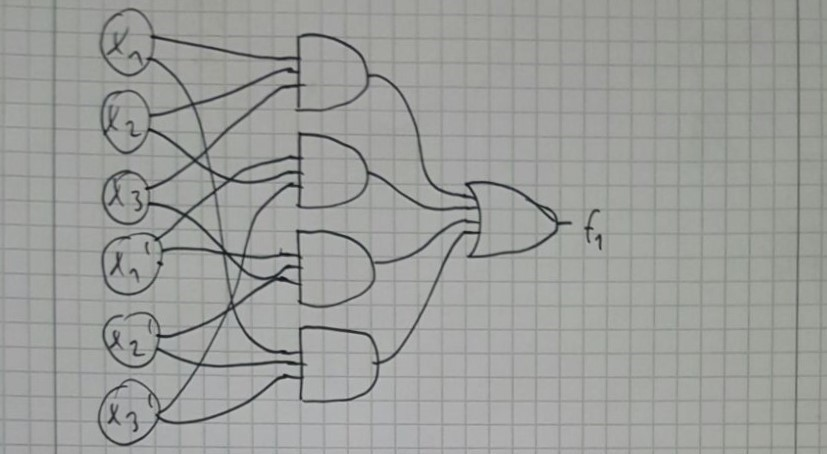
\includegraphics[width=13.6cm]{bild2.jpg}
		\item[c)] Schaltkreisbeschreibung:
		$ C := (\overrightarrow{X_{6}}, (V,E), typ, IN, \overrightarrow{Y_{1}}), $\\
		wobei\\
		$ V = \{0,1\} \cup \{x_{1}, x_{2}, x_{3}, x_{1}', x_{2}', x_{3}'\} \cup \{v_{0}, v_{1}, v_{2}, v_{3}, v_{4}\} $\\
		$ E = \{(x_{1},v_{0}), (x_{2},v_{0}), (x_{3},v_{0}), 
		(x_{1}',v_{1}), (x_{2},v_{1}), (x_{3}',v_{1}), 
		(x_{1}',v_{2}), (2_{2}',v_{2}), (x_{3},v_{2}), 
		(x_{1},v_{3}), (x_{2}',v_{3}),\\ (x_{3}',v_{3}), 
		(v_{0},v_{4}), (v_{1},v_{4}), (v_{2},v_{4}), (v_{3},v_{4})\} $ \\
		$ \overrightarrow{X_{6}} = (x_{1}, x_{2}, x_{3}, x_{1}', x_{2}', x_{3}') $ \\
		$ \overrightarrow{Y_{1}} = (v_{4}) $ \\
		$ typ = \{(v_{i} \mapsto \wedge) | i \in \{0,1,2,3\}\} \cup \{(v_{4} \mapsto \vee)\}$ \\
		$ IN = \{(v_{0} \mapsto ((x_{1}, v_{0}),(x_{2}, v_{0}),(x_{3}, v_{0}))), (v_{1} \mapsto ((x_{1}', v_{1}), (x_{2}, v_{1}), (x_{3}', v_{1}))), \\(v_{2} \mapsto ((x_{1}', v_{2}),(x_{2}', v_{2}),(x_{3}, v_{2}))), (v_{3} \mapsto ((x_{1}, v_{3}),(x_{2}', v_{3}),(x_{3}', v_{3}))), \\(v_{4} \mapsto ((v_{0}, v_{4}),(v_{1}, v_{4}),(v_{2}, v_{4}),(v_{3}, v_{4})))\} $.
		
	\end{itemize}
	\subsection*{Aufgabe 3}
	\begin{itemize}
		\item[a)]
		[Bild 3]\\
		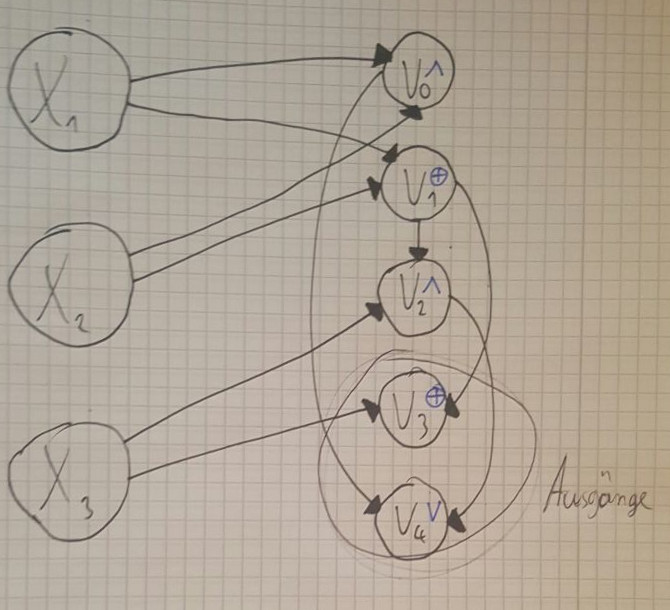
\includegraphics[width=14cm]{bild3.jpg}
		\item[b)] Funktionen der Gatter:\\
		
		\begin{table}[h]
			\begin{tabular}{l|l}
				Gatter & Funktion \\ \hline
				$v_{0}$ & $x_{1} \wedge x_{2}$ \\
				$v_{1}$ & $x_{1} \oplus x_{3}$ \\
				$v_{2}$ & $v_{1} \wedge x_{3}$ \\
				$v_{3}$ & $v_{1} \oplus x_{3}$ \\
				$v_{4}$ & $v_{0} \vee v_{2}$ \\
			\end{tabular}
		\end{table}
		
	\end{itemize}
	\subsection*{Aufgabe 4}
	\begin{itemize}
		\item[a)] 
		$f_1 = x_1'x_2'x_3'x_4 + x_1x_2'x_3'x_4  + x_1x_2'x_3x_4  + x_1x_2'x_3x_4' + x_1x_2x_3'x_4 + x_1x_2x_3x_4$ \\
		$f_2 = x_1'x_2'x_3x_4  + x_1'x_2x_3'x_4' + x_1'x_2x_3'x_4 + x_1'x_2x_3x_4 + x_1x_2x_3'x_4 + x_1x_2x_3x_4$
		\item[b)] [Cube 1 für $ON(f_1)$] \\
		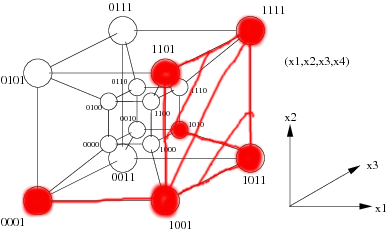
\includegraphics[width=14cm]{hypercube1.png}
		[Cube 2 für $ON(f_2)$] \\
		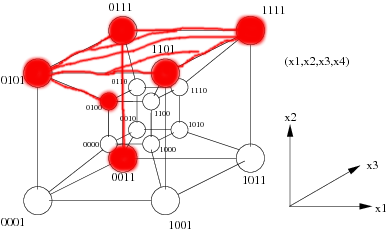
\includegraphics[width=14cm]{hypercube2.png}
		
		\item[c)] $g_1 = x_1x_4 + x_2'x_3'x_4 + x_1x_2'x_3 $ \\
		\\
		$g_2 = x_2x_4 + x_1'x_2x_3' + x_1'x_3x_4 $
		
	\end{itemize}
	
\end{document}
